\begin{frame}
    \frametitle{Introduction}
    \begin{block}{}
        \begin{itemize}
            \item We will take you through successfully launching a rocket and landing it on a different body
            \item This is a simplified version based on our knowledge of KSP not real life per se
        \end{itemize}
    \end{block}
\end{frame}
\begin{frame}
    \frametitle{Technicallities}
    \begin{block}{Jargon}
        \begin{description}
            \item [Orbit] An object rotating around another object is said to be in orbit
            \item [Inclined] An orbit that is tilted relative to the plane of the parent body
        \end{description}
    \end{block}
\end{frame}
\begin{frame}
    \frametitle{Technicallities}
    \begin{block}{delta-v}
        \begin{itemize}
            \item aka: fuel budget
            \item how hard can i accelerate/decelerate my rocket
            \item dependent on:
            \begin{itemize}
                \item fuel efficiency
                \item thurst to weight ratio
            \end{itemize}
        \end{itemize}
    \end{block}
\end{frame}
\begin{frame}
    \frametitle{Technicallities}
    \begin{block}{Points on orbit}
        \begin{description}
            \item[apoapsis]: highest point on orbit
            \item[periapsis]: Lowest point on orbit
        \end{description}
    \end{block}
    \begin{block}{}
        \begin{center}
            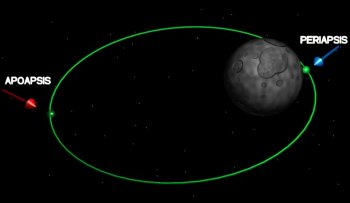
\includegraphics[scale=0.6]{images/apoapsis_periapsis.jpg}
        \end{center}
    \end{block}
\end{frame}
